\documentclass[12pt,letterpaper]{article}
\usepackage{graphicx,textcomp}
\usepackage{natbib}
\usepackage{setspace}
\usepackage{fullpage}
\usepackage{color}
\usepackage[reqno]{amsmath}
\usepackage{amsthm}
\usepackage{fancyvrb}
\usepackage{amssymb,enumerate}
\usepackage[all]{xy}
\usepackage{endnotes}
\usepackage{lscape}
\newtheorem{com}{Comment}
\usepackage{float}
\usepackage{hyperref}
\newtheorem{lem} {Lemma}
\newtheorem{prop}{Proposition}
\newtheorem{thm}{Theorem}
\newtheorem{defn}{Definition}
\newtheorem{cor}{Corollary}
\newtheorem{obs}{Observation}
\usepackage[compact]{titlesec}
\usepackage{dcolumn}
\usepackage{tikz}
\usetikzlibrary{arrows}
\usepackage{multirow}
\usepackage{xcolor}
\newcolumntype{.}{D{.}{.}{-1}}
\newcolumntype{d}[1]{D{.}{.}{#1}}
\definecolor{light-gray}{gray}{0.65}
\usepackage{url}
\usepackage{listings}
\usepackage{color}
\definecolor{codegreen}{rgb}{0,0.6,0}
\definecolor{codegray}{rgb}{0.5,0.5,0.5}
\definecolor{codepurple}{rgb}{0.58,0,0.82}
\definecolor{backcolour}{rgb}{0.95,0.95,0.92}

\lstdefinestyle{mystyle}{
	backgroundcolor=\color{backcolour},   
	commentstyle=\color{codegreen},
	keywordstyle=\color{magenta},
	numberstyle=\tiny\color{codegray},
	stringstyle=\color{codepurple},
	basicstyle=\footnotesize,
	breakatwhitespace=false,         
	breaklines=true,                 
	captionpos=b,                    
	keepspaces=true,                 
	numbers=left,                    
	numbersep=5pt,                  
	showspaces=false,                
	showstringspaces=false,
	showtabs=false,                  
	tabsize=2
}
\lstset{style=mystyle}
\newcommand{\Sref}[1]{Section~\ref{#1}}
\newtheorem{hyp}{Hypothesis}

\title{Problem Set 1  Applied Stats/Quant Methods 1}
\date{Due: September 30, 2024}
\author{Zengyuan Zhao/zhaoze@tcd.ie}

\begin{document}
	\maketitle
	
	\section*{Instructions}
	\begin{itemize}
	\item Please show your work! You may lose points by simply writing in the answer. If the problem requires you to execute commands in \texttt{R}, please include the code you used to get your answers. Please also include the \texttt{.R} file that contains your code. If you are not sure if work needs to be shown for a particular problem, please ask.
\item Your homework should be submitted electronically on GitHub.
\item This problem set is due before 23:59 on Monday September 30, 2024. No late assignments will be accepted.
%\item Total available points for this homework is 80.
	\end{itemize}
	
	\vspace{1cm}
	\section*{Question 1: Education}

A school counselor was curious about the average of IQ of the students in her school and took a random sample of 25 students' IQ scores. The following is the data set:\\
\vspace{.5cm}

\lstinputlisting[language=R, firstline=36, lastline=36]{PS01.R}  

\vspace{1cm}

\begin{enumerate}
	\item Find a 90\% confidence interval for the average student IQ in the school.\\
	\lstinputlisting[language=R, firstline=1, lastline=19]{PS01_answersZYZ.R}  
"The confidence interval is: (93.9599275120757, 102.920072487924)"\\
	\item Next, the school counselor was curious  whether  the average student IQ in her school is higher than the average IQ score (100) among all the schools in the country.\\ 
	\noindent Using the same sample, conduct the appropriate hypothesis test with $\alpha=0.05$.\\
	\lstinputlisting[language=R, firstline=21, lastline=36]{PS01_answersZYZ.R}
	"The average IQ of students in this school is not higher than the national average."\\
\end{enumerate}


	\section*{Question 2: Political Economy}

\noindent Researchers are curious about what affects the amount of money communities spend on addressing homelessness. The following variables constitute our data set about social welfare expenditures in the USA. \\
\vspace{.5cm}


\begin{tabular}{r|l}
	\texttt{State} &\emph{50 states in US} \\
	\texttt{Y} & \emph{per capita expenditure on shelters/housing assistance in state}\\
	\texttt{X1} &\emph{per capita personal income in state} \\
	\texttt{X2} &  \emph{Number of residents per 100,000 that are "financially insecure" in state}\\
	\texttt{X3} &  \emph{Number of people per thousand residing in urban areas in state} \\
	\texttt{Region} &  \emph{1=Northeast, 2= North Central, 3= South, 4=West} \\
\end{tabular}

\vspace{.5cm}
\noindent Explore the \texttt{expenditure} data set and import data into \texttt{R}.
\vspace{.5cm}
\lstinputlisting[language=R, firstline=54, lastline=54]{PS01.R}  
\vspace{.5cm}
\begin{itemize}

\item
Please plot the relationships among \emph{Y}, \emph{X1}, \emph{X2}, and \emph{X3}? What are the correlations among them (you just need to describe the graph and the relationships among them)?
\vspace{1cm}
\lstinputlisting[language=R, firstline=38, lastline=102]{PS01_answersZYZ.R}
\begin{figure}[h!]\centering
	\caption{\footnotesize YvsX1 scatterplot.}
	\label{fig:plot_Y_vs_X1}
	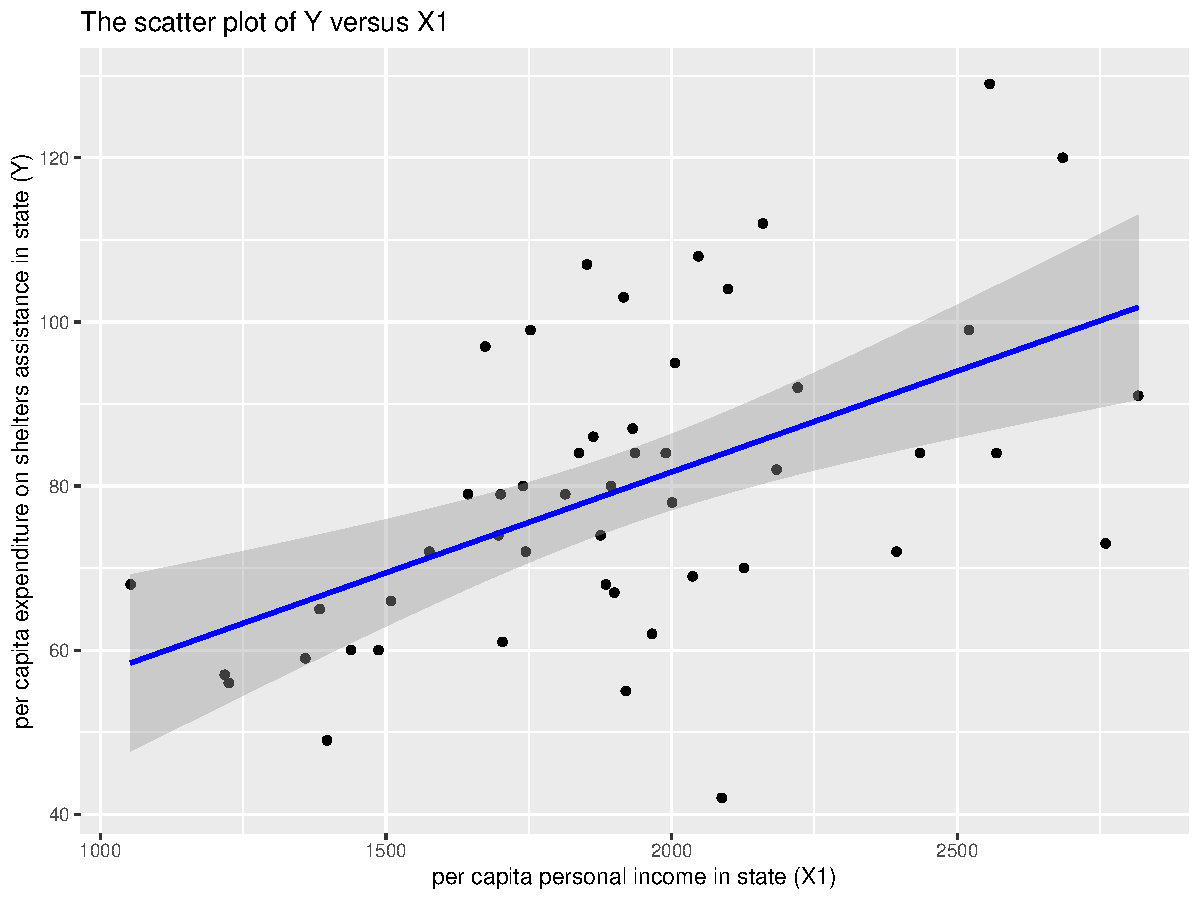
\includegraphics[width=.75\textwidth]{Y_vs_X1_scatterplot.pdf}
\end{figure}
\begin{figure}[h!]\centering
	\caption{\footnotesize YvsX2 scatterplot.}
	\label{fig:plot_Y_vs_X2}
	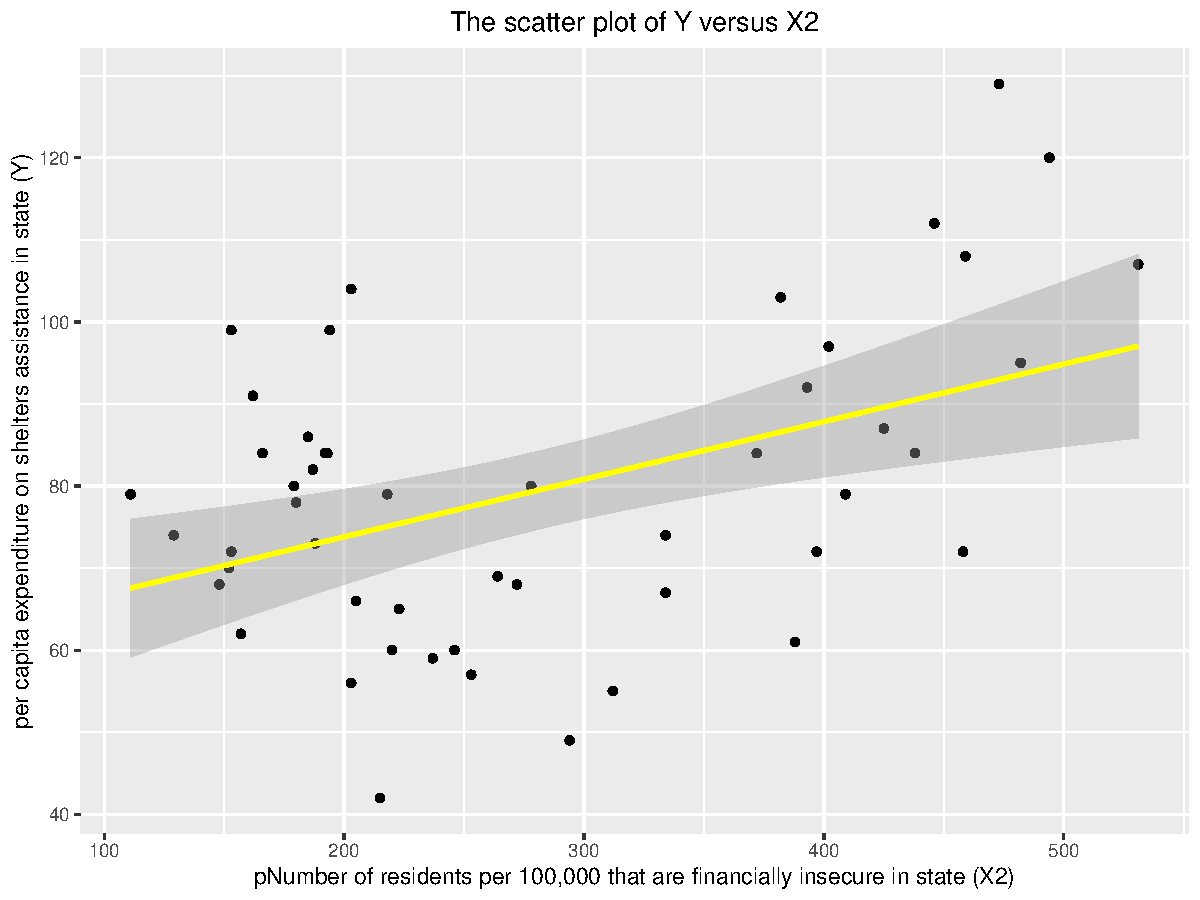
\includegraphics[width=.75\textwidth]{Y_vs_X2_scatterplot.pdf}
\end{figure}
\begin{figure}[h!]\centering
	\caption{\footnotesize YvsX3 scatterplot.}
	\label{fig:plot_1Y_vs_X3}
	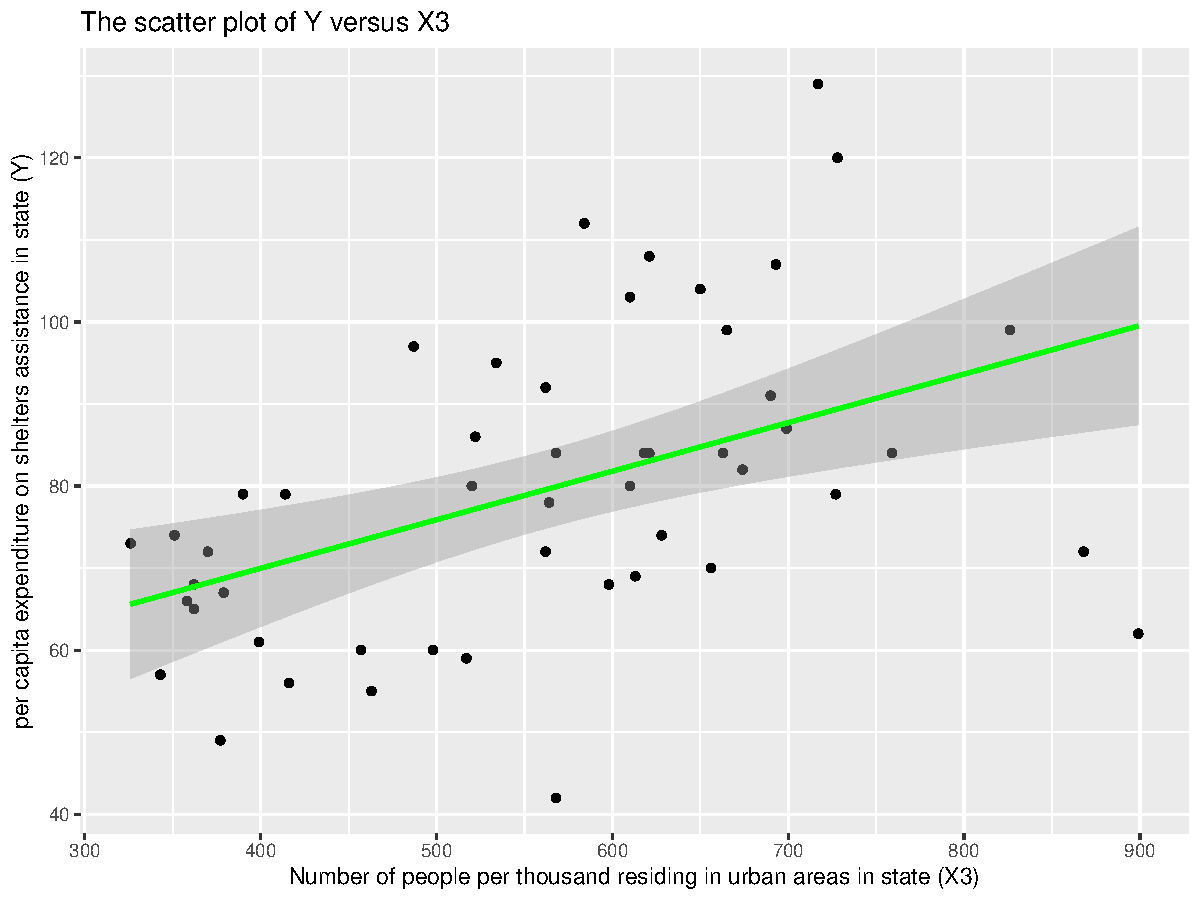
\includegraphics[width=.75\textwidth]{Y_vs_X3_scatterplot.pdf}
\end{figure}
\begin{figure}[h!]\centering
	\caption{\footnotesize X1vsX2 scatterplot.}
	\label{fig:plot_X1_vs_X2}
	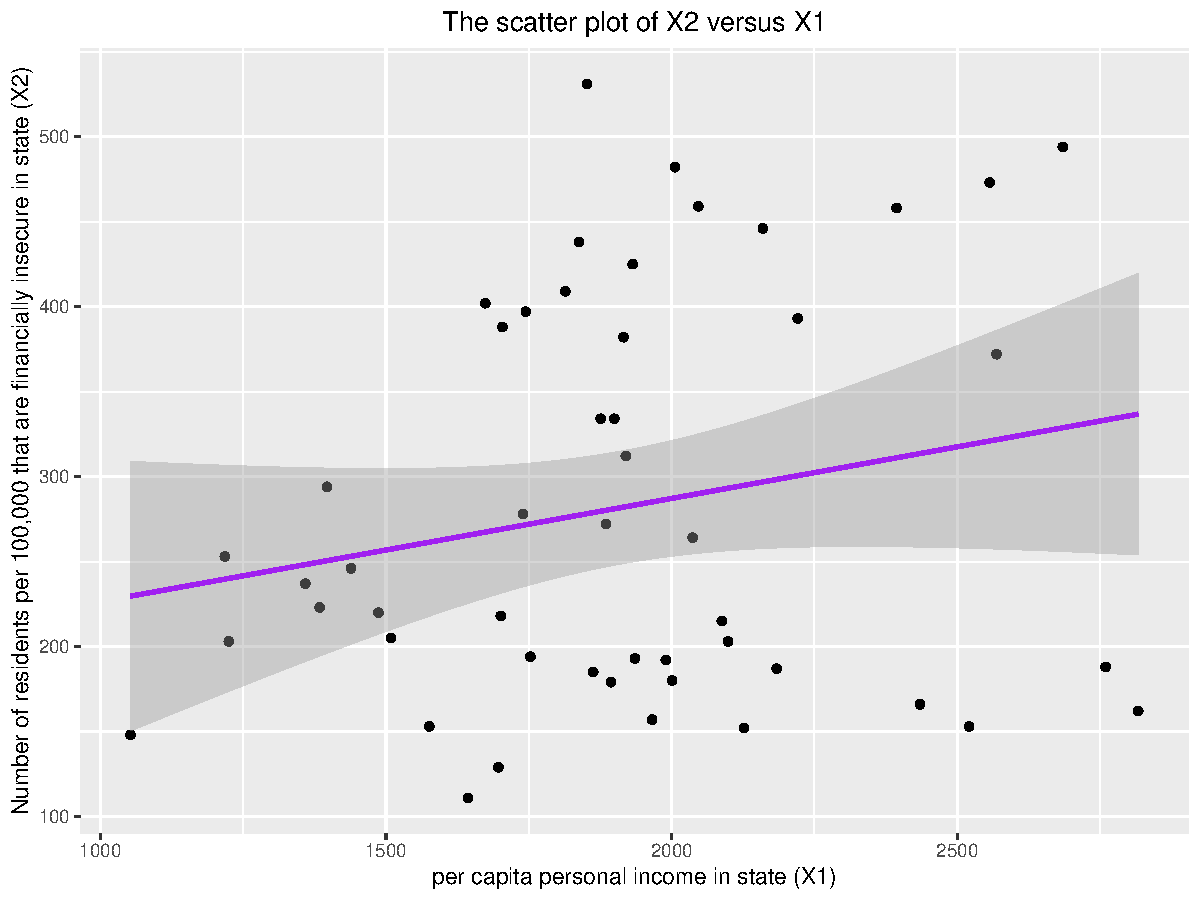
\includegraphics[width=.75\textwidth]{X1_vs_X2_scatterplot.pdf}
\end{figure}
\begin{figure}[h!]\centering
	\caption{\footnotesize X1vsX3 scatterplot.}
	\label{fig:plot_X1_vs_X3}
	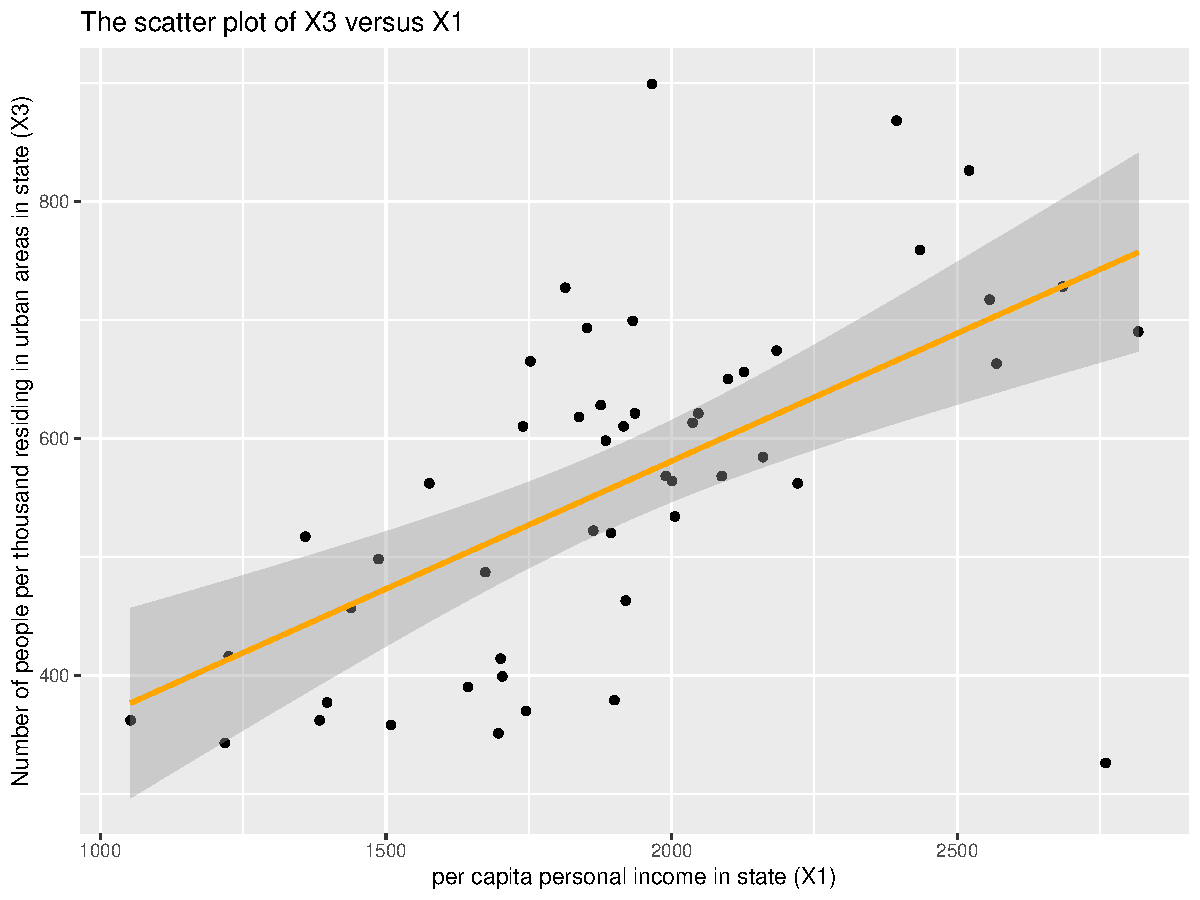
\includegraphics[width=.75\textwidth]{X1_vs_X3_scatterplot.pdf}
\end{figure}
\begin{figure}[h!]\centering
	\caption{\footnotesize X2vsX3 scatterplot.}
	\label{fig:plot_X2_vs_X3}
	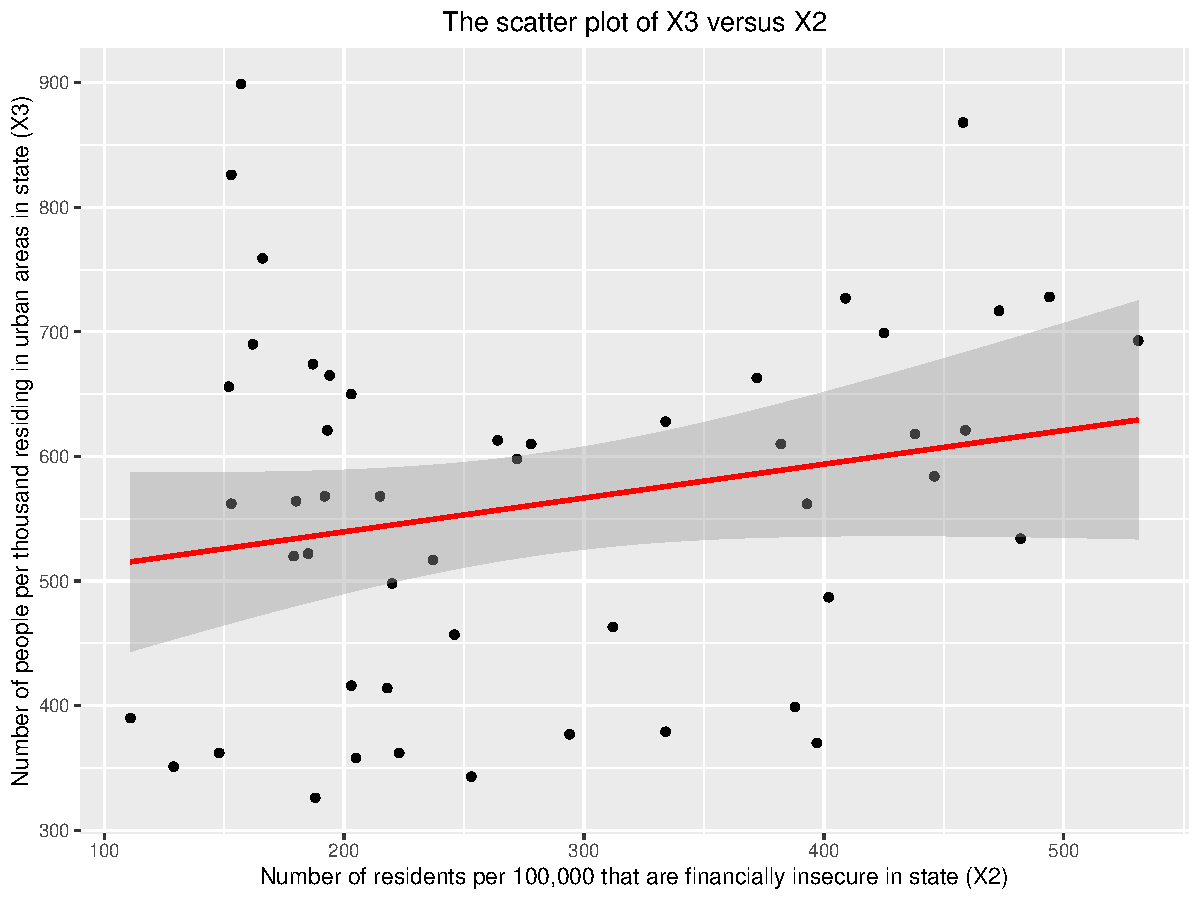
\includegraphics[width=.75\textwidth]{X2_vs_X3_scatterplot.pdf}
\end{figure}
\begin{figure}[h!]\centering
	\caption{\footnotesize  scatterplot matrix}
	\label{fig:matrix_X1_X2_X3_X4_Y}
	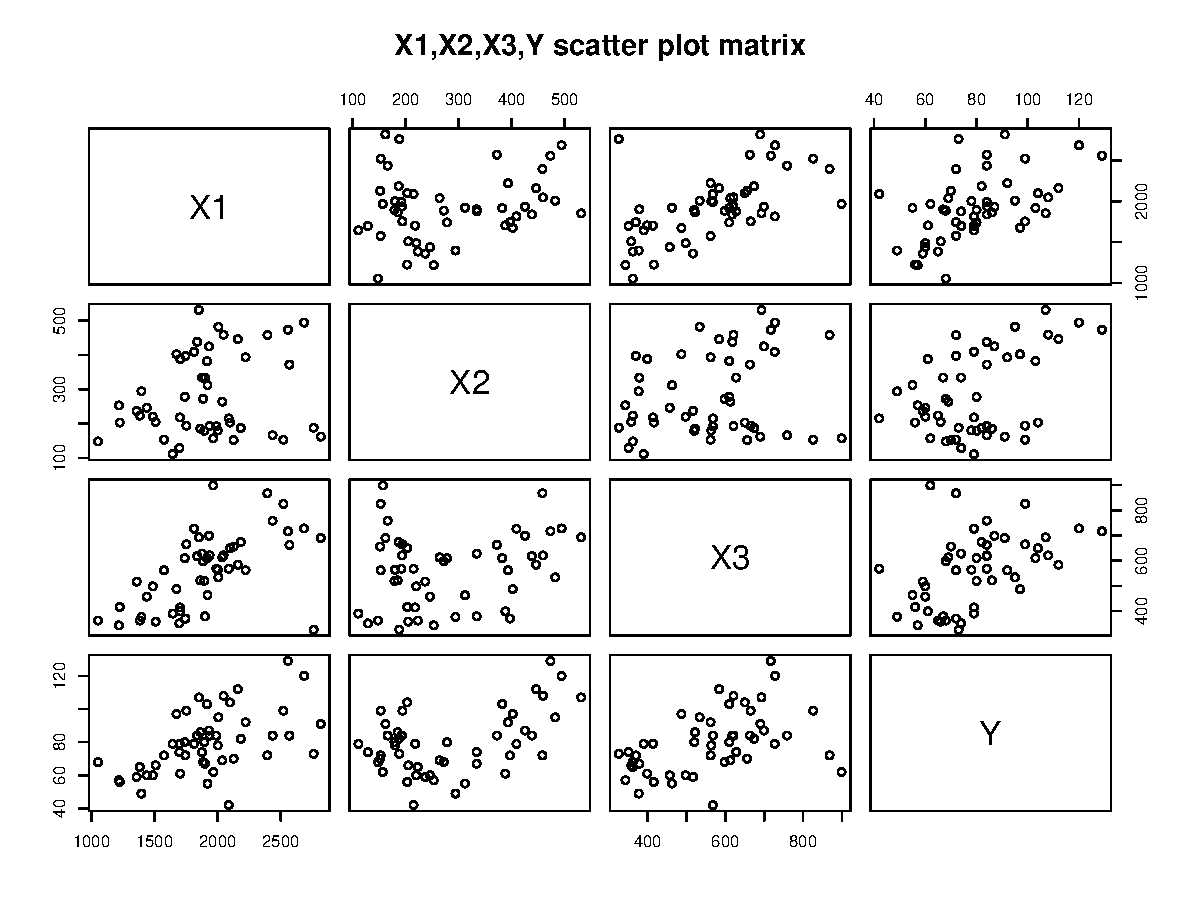
\includegraphics[width=.75\textwidth]{scatterplot_matrix.pdf}
\end{figure}
\vspace{10cm}
 From the above six scatter plots between X1, X2, X3 and Y and the linear model smooth line, we can know that there is a positive correlation between X1, X2, X3 and Y. Among them, there is a strong positive correlation between Y and X1, which shows that the more personal income in each region, the more investment in assisted housing, and vice versa. X1 and X3 also have a strong positive correlation, which shows that the more individuals in each region earn more, the greater the proportion of people living in urban areas.The correlation between X2 and X3 is weak, indicating that the number of "financially insecure" residents per 100,000 people in the state has little to do with the number of people living in urban areas. \\
\end{itemize}
\vspace{1cm}
\begin{itemize}
\item
Please plot the relationship between \emph{Y} and \emph{Region}? On average, which region has the highest per capita expenditure on housing assistance?
\lstinputlisting[language=R, firstline=104, lastline=129]{PS01_answersZYZ.R}
\vspace{.5cm}
\begin{figure}[h!]\centering
	\caption{\footnotesize Region2vsY2 scatterplot}
	\label{fig:Region2_vs_Y2}
	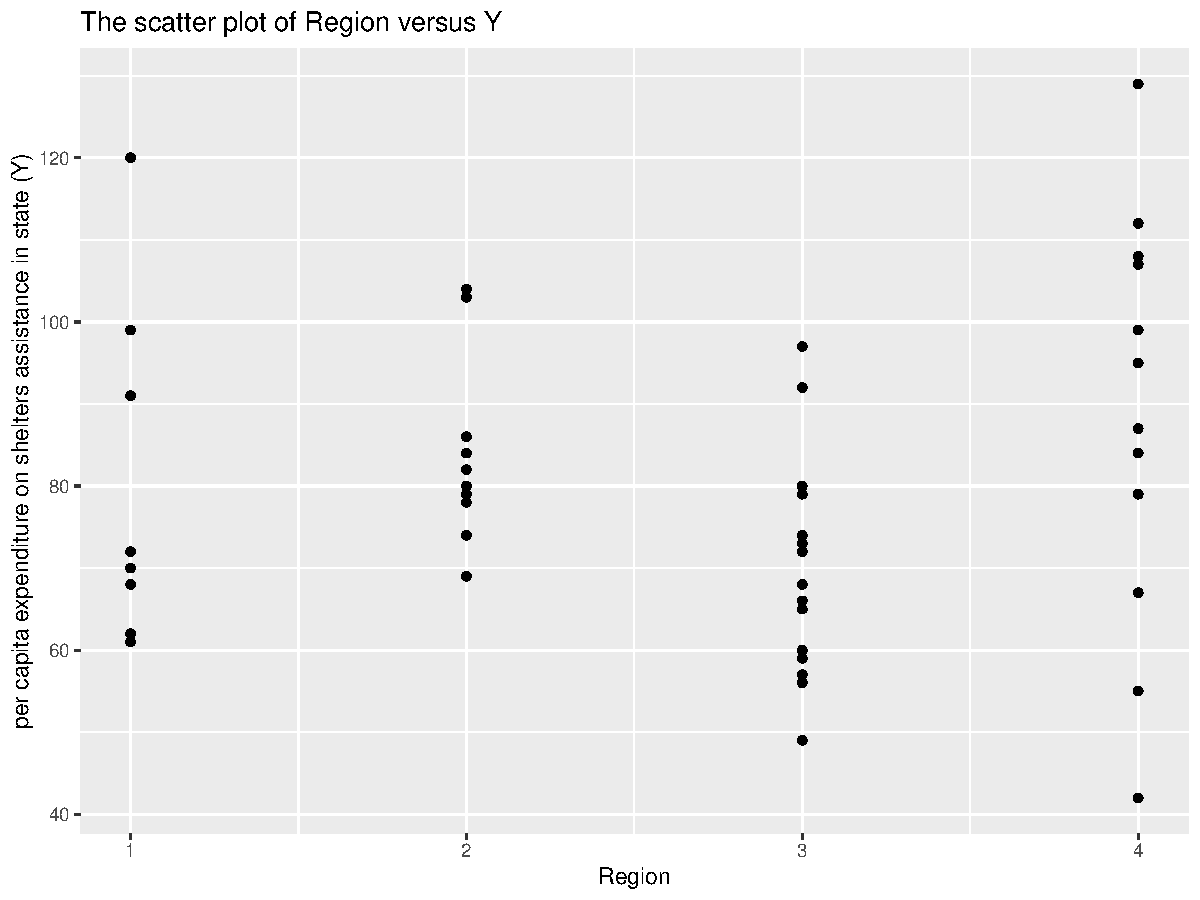
\includegraphics[width=.75\textwidth]{Region2_vs_Y2_scatterplot.pdf}
\end{figure}
\begin{figure}[h!]\centering
	\caption{\footnotesize Region2vsY2 scatterplot}
	\label{fig:Region1_vs_Y1}
	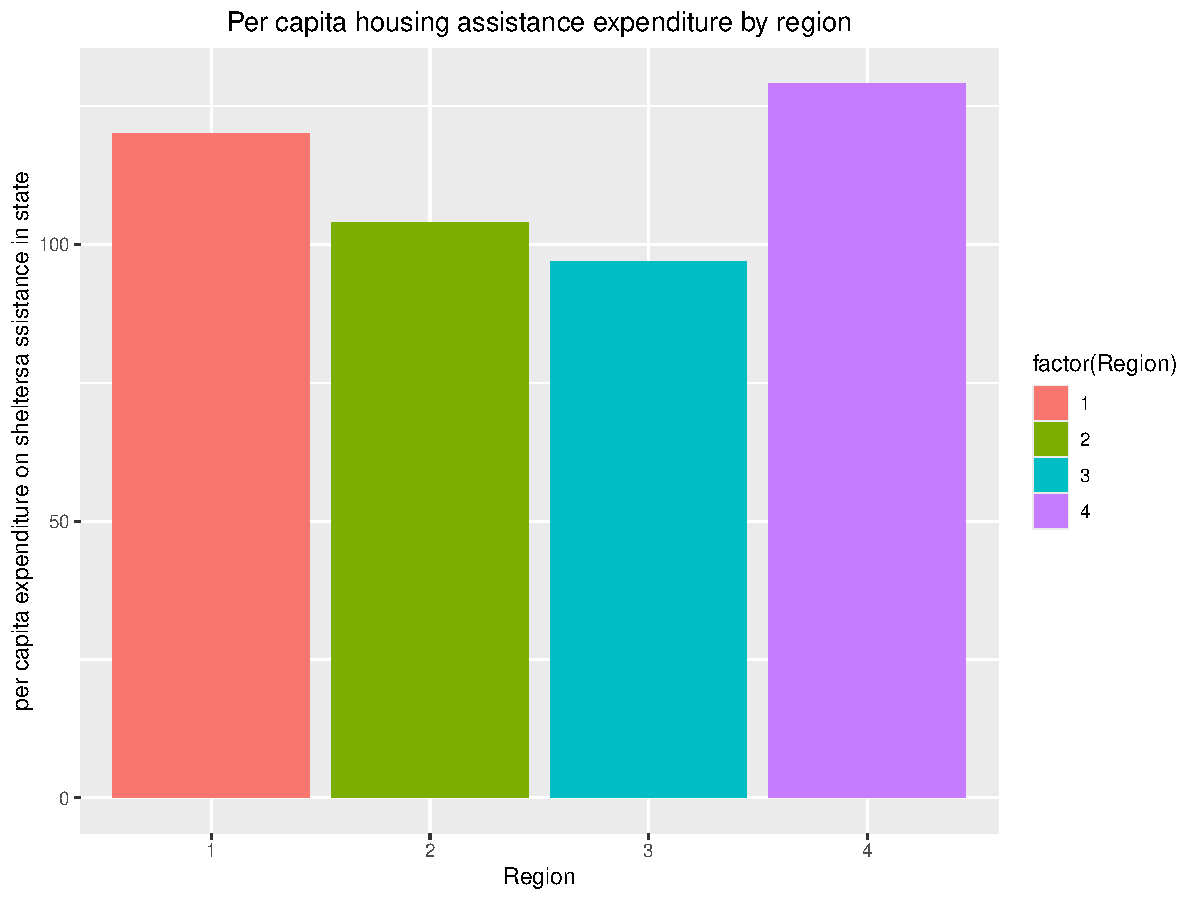
\includegraphics[width=.75\textwidth]{Region1_vs_Y1_barchart.pdf}
\end{figure}
\begin{figure}[h!]\centering
	\caption{\footnotesize model summary}
	\label{fig:regression model}
	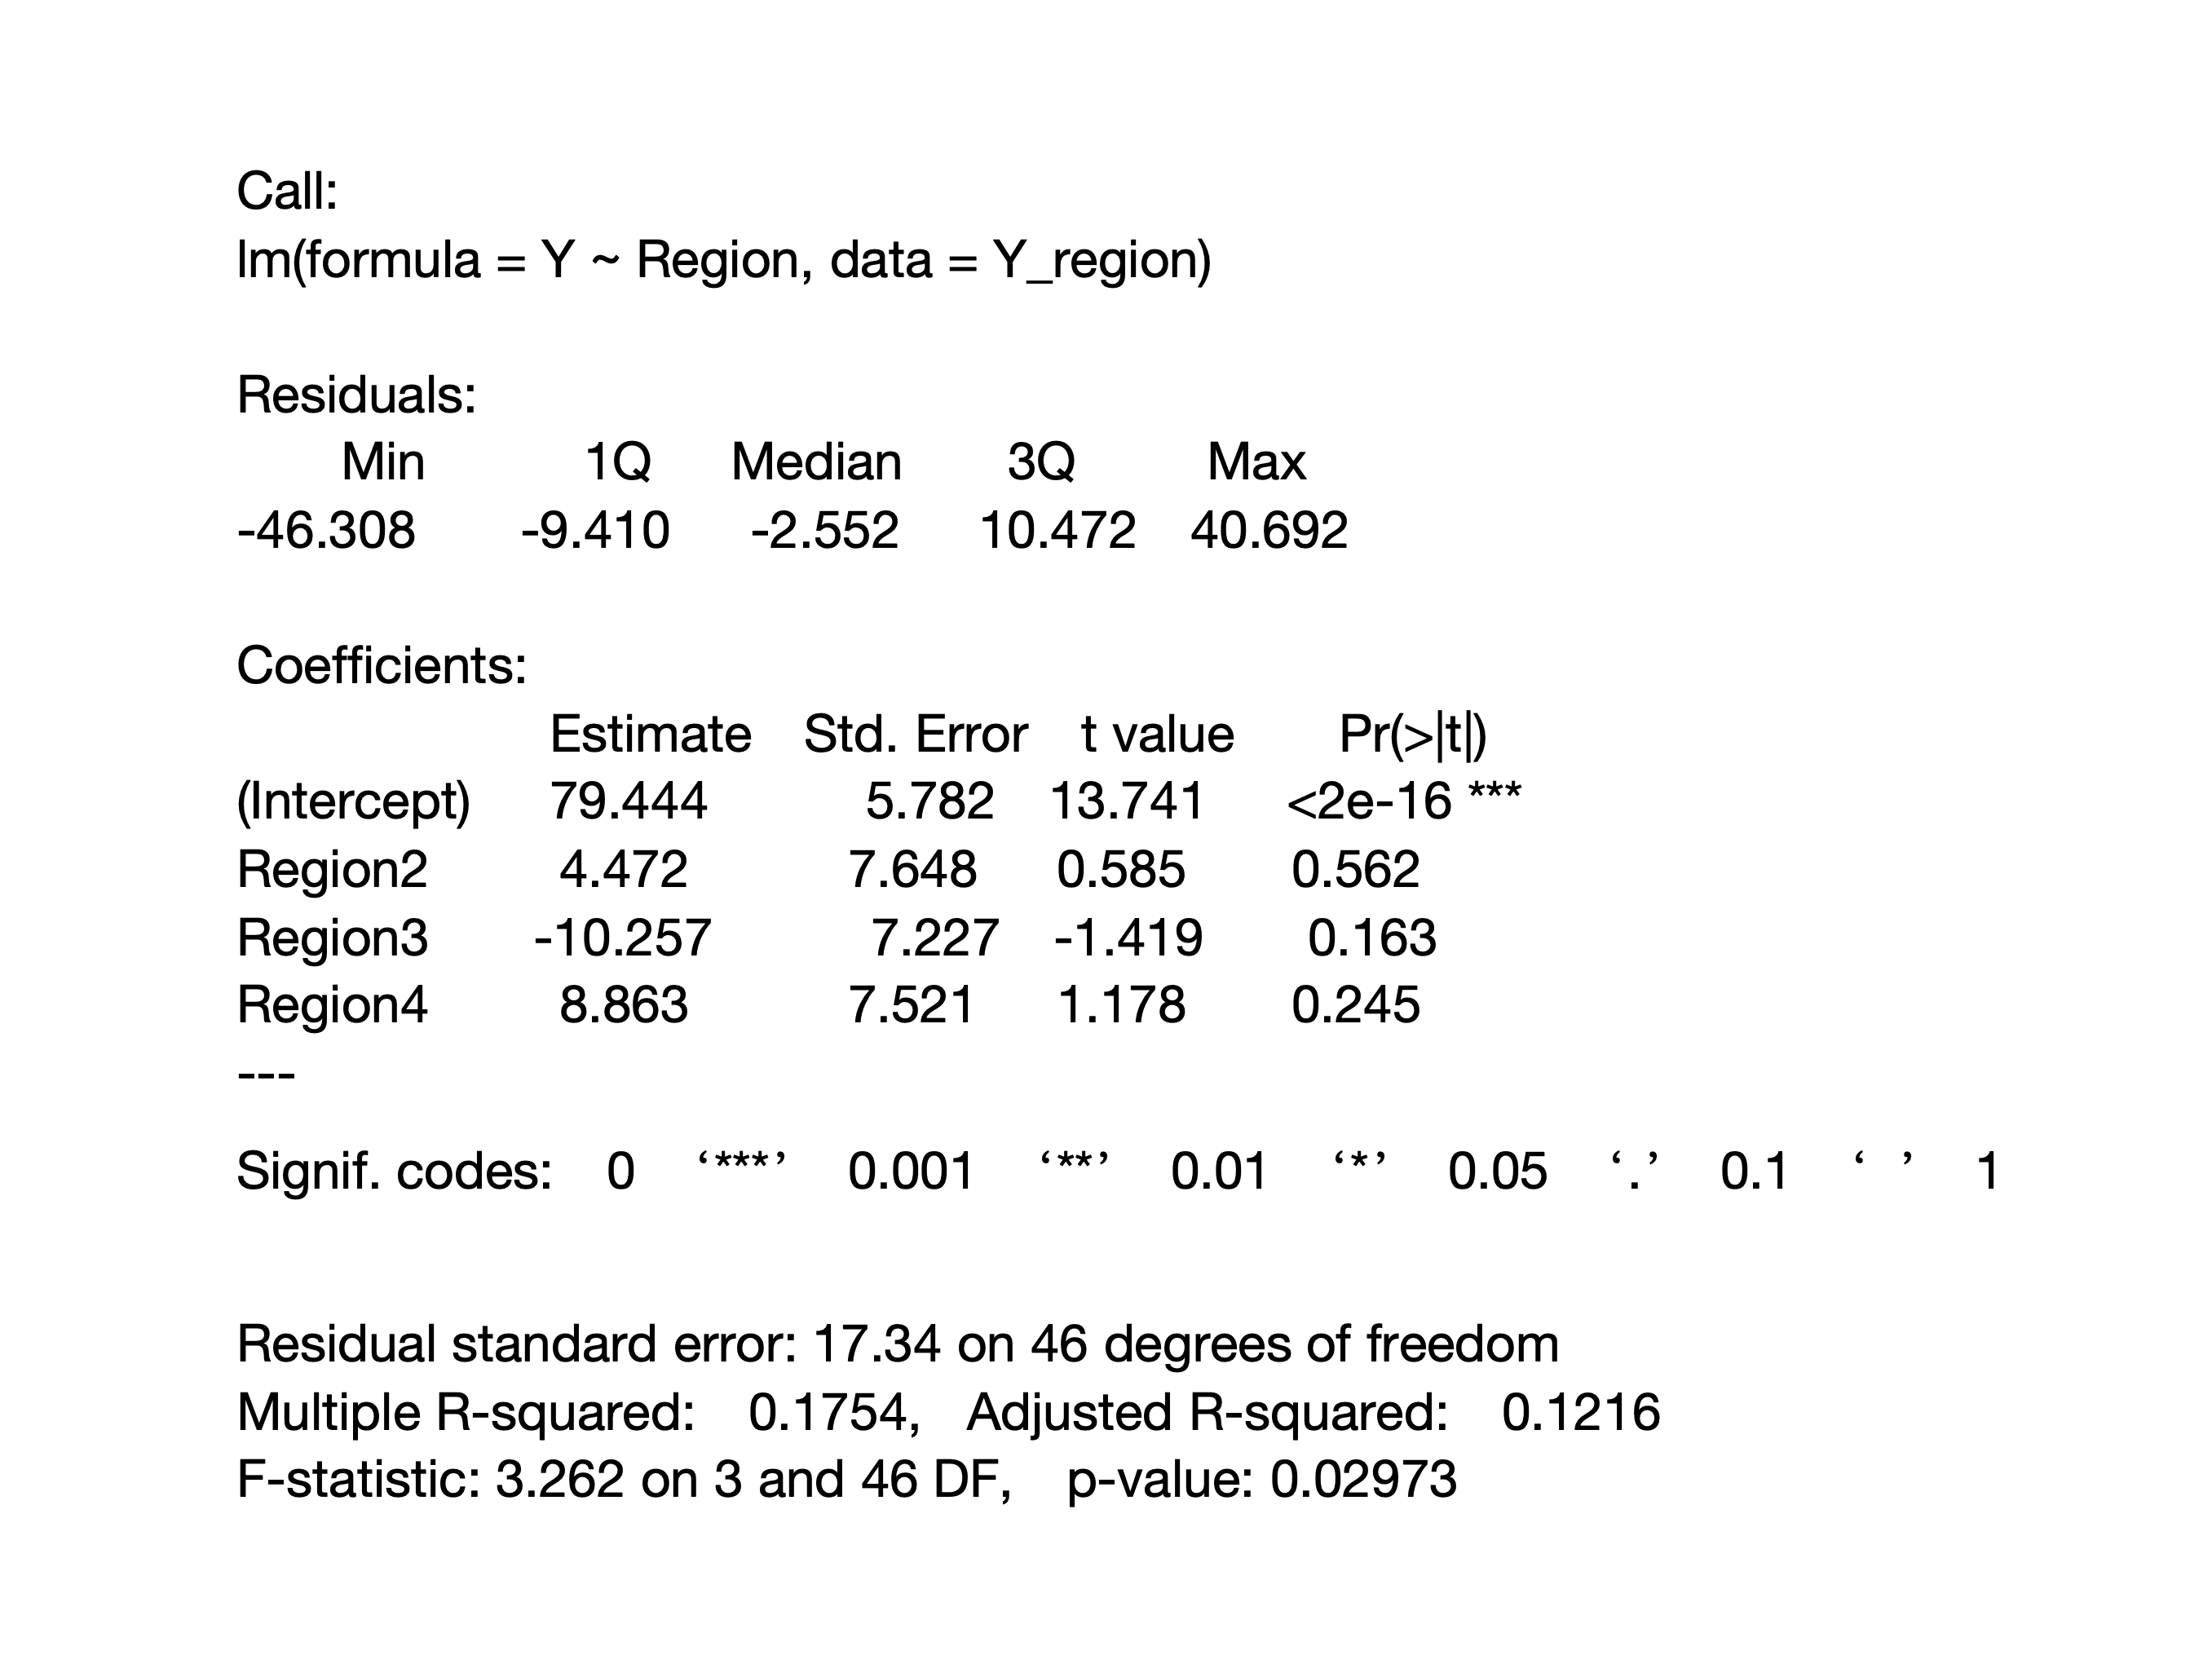
\includegraphics[width=.75\textwidth]{model.png}
\end{figure}
\vspace{10cm}
The p-value of the F statistic is 0.02973, which is less than the commonly used significance level of 0.05, which indicates that the Region variable has a significant impact on Y as a whole. From the scatter plot, the data points in the North Central region are concentrated and may have a strong correlation. On average, the western region has the highest spending on housing support, at about 88.30769.\\
\item
Please plot the relationship between \emph{Y} and \emph{X1}? Describe this graph and the relationship. Reproduce the above graph including one more variable \emph{Region} and display different regions with different types of symbols and colors.
\lstinputlisting[language=R, firstline=131, lastline=143]{PS01_answersZYZ.R}
\vspace{1cm}
\begin{figure}[h!]\centering
	\caption{\footnotesize X1vsYvsRegion scatterplot}
	\label{fig:X1vsY_Region}
	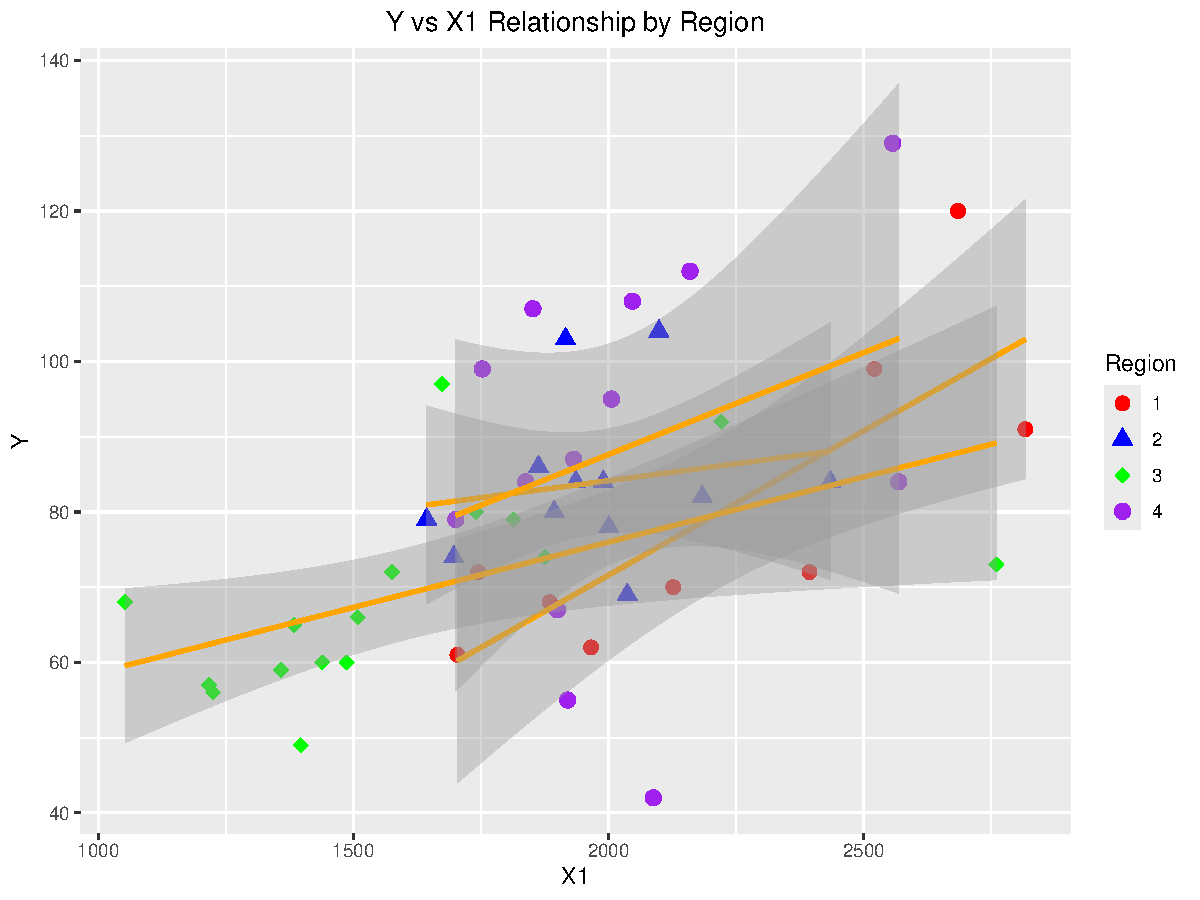
\includegraphics[width=.75\textwidth]{X1vsY_Region_scatterplot.pdf}
\end{figure}
From this scatter plot, we can see that the per capita income of each region and the expenditure on housing support are positively correlated, and the correlation coefficient is 0.5317212, which is a strong positive correlation. In addition, the correlation between personal income and expenditure on housing support in the Northeast region (Region 1) is stronger than in other regions.\\
\end{itemize}


\end{document}
